\ifx \globalmark \undefined %% This is default.
	\documentclass[twoside,openright,11pt,a4paper]{report}

%\compiler avec xelatex
%\usepackage[applemac]{inputenc}
\usepackage[T1]{fontenc}
\usepackage[utf8]{inputenc} %latin1 est possible
%\usepackage[latin1]{inputenc} %latin1 est possible
\usepackage[UKenglish]{babel}
\usepackage{lettrine}

%\usepackage[text={13cm,20cm},centering]{geometry}
\usepackage [squaren, Gray, mediumqspace]{SIunits}
\usepackage [top=2cm, bottom=2cm, left=2cm, right=2cm ]{geometry}

\renewcommand{\familydefault}{cmss}
\addto\captionsenglish{ \renewcommand\chaptername{Solutions of Chapte}}

\usepackage{graphicx}
\usepackage{amsmath}
\usepackage{amsfonts}
\usepackage{amssymb}
\usepackage{amsthm}
\usepackage{bm}
\usepackage{color}

\newcommand{\real}{\mathbb{R}}
\newcommand{\mb}{\mathbf}
\newcommand{\bos}{\boldsymbol}

\def \RR {I \! \! R}

\newcommand{\e}{\begin{equation}}  
\newcommand{\ee}{\end{equation}}
\newcommand{\eqn}{\begin{eqnarray}} 
\newcommand{\eeqn}{\end{eqnarray}} 
\newcommand{\eqnn}{\begin{eqnarray*}} 
\newcommand{\eeqnn}{\end{eqnarray*}} 

\newcommand{\bpm}{\begin{pmatrix}}
\newcommand{\epm}{\end{pmatrix}}

%\newcommand{\{\c c}}{\c c}

\newcommand{\bma}{\left(\begin{array}}
\newcommand{\ema}{\end{array}\right)} 
\newcommand{\hh}{\hspace{2mm}}
\newcommand{\hd}{\hspace{5mm}}
\newcommand{\hu}{\hspace{1cm}}
\newcommand{\vv}{\vspace{2mm}}
\newcommand{\vd}{\vspace{5mm}}
\newcommand{\vm}{\vspace{-2mm}}
\newcommand{\teq}{\triangleq}
%\newcommand{\qedb}{\,$\Box$}
\newcommand{\blanc}{$\left. \right.$}
\newcommand{\frts}[2]%
         {\frac{{\textstyle #1}}{{\textstyle #2}}}

\newcommand{\bindex}[3]%
{
\renewcommand{\arraystretch}{0.5}
\begin{array}[t]{c}
#1\\
{\scriptstyle #2}\\
{\scriptstyle #3}
\end{array}
\renewcommand{\arraystretch}{1}
}

\theoremstyle{definition}
\newtheorem{exemple}{{\bf Exemple}}[chapter]
\newtheorem{theoreme}[exemple]{{\bf Th{é}or{è}me}}
\newtheorem{propriete}[exemple]{{\bf Propri{é}t{é}}}
\newtheorem{definition}[exemple]{{\bf D{é}finition}}
\newtheorem{remarque}[exemple]{{\bf Remarque}}
\newtheorem{remarques}[exemple]{{\bf Remarques}}
\newtheorem{lemme}[exemple]{{\bf Lemme}}
\newtheorem{hypothese}[exemple]{{\bf Hypoth{è}se}}
\newtheorem{exercice}{{\bf Exercice}}[chapter]

\newcommand{\xqedhere}[2]{%
 \rlap{\hbox to#1{\hfil\llap{\ensuremath{#2}}}}}

\newcommand{\xqed}[1]{%
 \leavevmode\unskip\penalty9999 \hbox{}\nobreak\hfill
 \quad\hbox{\ensuremath{#1}}}

\newcommand{\gf}{\fg\,\,}

\newcommand{\cata}[1] %
     {\renewcommand{\arraystretch}{0.5}
     \begin{array}[t]{c} \longrightarrow \\ {#1} \end{array}
     \renewcommand{\arraystretch}{1}}

\usepackage[isu]{caption}
%\usepackage[font=small,format=plain,labelfont=bf,up,textfont=it,up]{caption}
\setlength{\captionmargin}{60pt}

\newcommand{\cqfd}
{%
\mbox{}%
\nolinebreak%
\hfill%
\rule{2mm}{2mm}%
\medbreak%
\par%
}

\pagestyle{headings}

\renewcommand{\sectionmark}[1]{%
\markright{\thesection.\ #1}{}}

\renewcommand{\chaptermark}[1]{%
\markboth{\chaptername\ \thechapter.\ #1}{}}

\makeatletter 
\def\@seccntformat#1{\csname the#1\endcsname.\;} 
\makeatother

\title{ {\Huge {\textbf{Modélisation et analyse  \\ \vspace{4mm} des systèmes dynamiques }}} \\ \vspace{4cm} G. Bastin}

%\title{ {\Huge {\textbf{Modelisation et analyse  \\ \vspace{4mm} des systemes dynamiques }}} \\ \vspace{4cm} G. Bastin}


\date{\today}
	\begin{document} %% Crashes if put after (one of the many mysteries of LaTeX?).
\else 
	\documentclass{standalone}
	\begin{document}
\fi


\graphicspath{ {Chapitre4/images/} }

\setcounter{chapter}{3}
\chapter{Compartment systems}
\chaptermark{Compartment system}\label{syscompart}
%%%%%%%%%%%%%%%%%%%%%%%%%%%%%%%%%%%%%%%%%%%%%%%%%%
%%%%%%%%%%%%%%%%%%%%%%%%%%%%%%%%%%%%%%%%%%%%%%%%%%
%%%%%%%%%%%%%%%%%%%%%%%%%%%%%%%%%%%%%%%%%%%%%%%%%%
%%%%%%% PARTIE DE Nicolas Stevens    %%%%%%%%%%%%%%
%%%%%%%%%%%%%%%%%%%%%%%%%%%%%%%%%%%%%%%%%%%%%%%%%%
%%%%%%%%%%%%%%%%%%%%%%%%%%%%%%%%%%%%%%%%%%%%%%%%%%
%%%%%%%%%%%%%%%%%%%%%%%%%%%%%%%%%%%%%%%%%%%%%%%%%%
\lettrine[lines=1]{\bf T}{}he notion of compartment system is used to specify a wide set of systems for which the dynamic can be described  by balanced equations.
It is used in many engineering fields (such as chemistry engineering, biomedical engineering or ecology), in economy and social sciences as well. 

\section{Definitions and notations}
A compartment is a conceptual tank or box for which the content (matter, energy, money, population...) can be quantified.
The symbolic notation used is depicted at figure \ref{fig:compartiment} 
where $q_{in}$ and $q_{out}$ are respectively the filling and emptying flows 
of the compartment expressed in quantity of content by time unit.
These flows are always {\em positive}, by convention.


\begin{figure}[ht]
\begin{center}
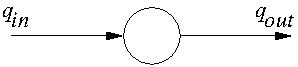
\includegraphics{compartiment}
\caption{Symbolic representation of the compartment.}
\label{fig:compartiment}
\end{center}
\end{figure}

A compartment system is made of one {\em network} of compartments 
interconnected and labelled $1$ through $n$.
To be clear, an example of system made of $3$ compartments is shown
at figure \ref{fig:exemplecomp}. The arrows specify the flows of content
exchanged by the the compartment in the network and with outside of 
the system.

\begin{figure}[ht]
\begin{center}
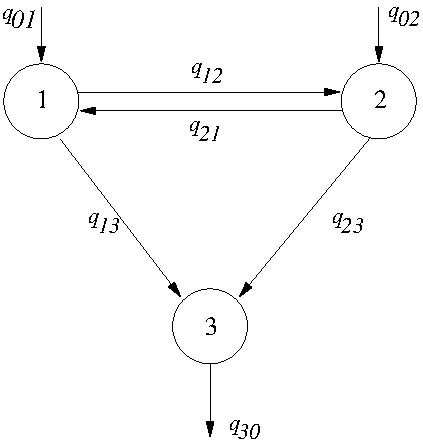
\includegraphics[width=5cm]{exemplecomp}
\caption{An example of a compartment system graph.}
\label{fig:exemplecomp}
\end{center} 
\end{figure}

In general, a compartment system is represented by an {\em oriented graph} 
whose nodes correspond to compartments and arcs to flows. 
The following notations are introduced~:
\begin{description}
\item $x_i$ is the quantity of content in the compartment of indices $i$,
$(i = 1, ... ,n)$. This quantity is always {\em positive}. Using a slight abuse of terms,
$x_i$ is used to depict the {\em level} of matter in the compartment $i$.
\item $q_{ij}$ specify the flow flowing from compartment $i$ towards the  
compartment $j$, $(i = 1, ... ,n ; j = 1, ... ,n)$. As mentioned above, it is a
variable which is always {\em positive} by convention.
\end{description}

\begin{definition}{\bf \em Open or close system}
A system is {\bf open} when there exists a possibility to exchange matter
with outside the system.
In this case :  
\begin{description}
\item $q_{io}$ specify the flow from  compartment $i$ towards the outside
\item $q_{oi}$ specify the flow from the outside towards the compartment $i$
\end{description}
Otherwise, the system is said to be {\bf close} : $q_{io} = 
q_{oi} = 0$ for all $i$. \qed
\end{definition}

\begin{definition}{\bf \em System connected to entrances and exits}

A compartment $i$ is {\it connected to an exit} if there is a path $i \rightarrow j \rightarrow k \rightarrow \dots \rightarrow \ell$ from this compartment ending in a compartment $\ell$ from which there is an outgoing flow  $q_{\ell o}$. The system is {\it completely connected to the exits} (CCO) if each and every compartment is connected to an exit.

A compartment $\ell$ is {\it connected to an entry} if there is a path $i \rightarrow j \rightarrow k \rightarrow \dots \rightarrow \ell$ ending in this compartment and coming from a compartment $i$ in which there is an entering flow $q_{oi}$. The system is {\it completely connected to the entries} (CCI) if every compartment is connected to an entry. \qed 
\end{definition}


\section{State model}
\markboth{ {\bf \hspace*{5mm}Chapter 4 }\hfill Compartment system} {{ \bf Sec. \thesection} \hfill
State model \hspace*{5mm}}

The balanced equation of every compartment (also called continuity equation)
\eqnn
\dot{x_i} = \sum_{j=0}^n q_{ji}(t) - \sum_{j=0}^n q_{ij}(t) \hspace{1cm} i=1,...,n
\label{bilan}
\eeqnn
is the basic statement to establish the state model of a compartment system.
This equation tells us that the variation, per unit of time, of the 
quantity contained in a compartment is the difference between the 
sum of the entering flows (or debits) and the sum of the outgoing flows (or debits). 
In practice, of course, the flows wich are structurely null are not explicitly in the equation  
(\eqref{bilan}).

Computing the equations of the sate model of a compartment system required two 
fundamental aspects. 

First of all, the structure of the graph related to the system determines the 
number and the structure of the balanced equations (\eqref{bilan}) ; the variables $x_i$ are
the state variables whereas the order of the model is the number $n$ of  
compartments.

To complete the state model, the flows should be specified in terms of the 
state variables and input variables : 
\eqnn
q_{ij}(x,u)
\eeqnn
where $x$ et $u$ are, as usual, the vector of state and entries. 
This modelling is the point of the next section.

The general form of the state equations of a compartment system is the 
following :  
\eqnn
\dot{x_i} = \sum_{j=0}^n q_{ji}(x,u) - \sum_{j=0}^n q_{ij}(x,u) \hspace{1cm} i=1,...,n \label{eqetcomp}
\eeqnn
In this model, the physical meaning of the state variables $x_i$ is obvious : these are
the quantities contained in each compartment. But, the input variables $u$ can be 
of different nature, depending on the applications, as the next examples will show.

If the {\em flows vector} $q(x,u)$ is defined as containing, in an arbitrary order, all the
flows $q_{ij}(x,u)$ which are not structurally null, then the sate model (\eqref{eqetcomp}) 
can also be written in a more compact matrix form :
\eqn
\dot{x} = Lq(x,u) \label{modetcomp}
\eeqn
where $L$ is the incident matrix of the oriented graph, whose  
coefficents all belong to 
$(-1,0,1)$, which is ?????.

\begin{exemple}
For the system depicted at figure \ref{fig:exemplecomp}, the
state model is written as :
\eqnn
\dot{x_1} &=& q_{01}(x,u) - q_{12}(x,u) - q_{13}(x,u) + q_{21}(x,u) \\
\dot{x_2} &=& q_{02}(x,u) + q_{12}(x,u) - q_{21}(x,u) - q_{23}(x,u) \\
\dot{x_3} &=& q_{13}(x,u) + q_{23}(x,u) - q_{30}(x,u)
\eeqnn
If the flows vector is defined as :
\eqnn
q(x,u) \triangleq \bma{c} q_{01}(x,u) \\ q_{02}(x,u) \\ q_{12}(x,u) \\
q_{13}(x,u) \\ q_{21}(x,u) \\ q_{23}(x,u) \\ q_{30}(x,u) \ema
\eeqnn
the state model is written in a matrix format (\eqref{modetcomp}) with  
the matrix $L$ :
\eqnn
L \triangleq \bma{ccccccc} 1 & 0 & -1 & -1 & 1 & 0 & 0 \\
0 & 1 & 1 & 0 & -1 & -1 & 0 \\
0 & 0 & 0 & 1 & 0 & 1 & -1 \ema.
\eeqnn
\qed
\end{exemple}

\section{Modelling of the flows}

Depending on the applications, the functions $q_{ij}(x,u)$ depicting the flows can take different types of
forms. However, they must be defined in a way which guarantees the compartment system to be a {\em positive system}, that is a system for which every state variable remains positive along the trajectories. 
It is a likelihood guarantee of the model, because the state variables represent measures which do not have a 
physical meaning if they are negative.

\begin{definition} \label{vecpositif} {\bf \em Positive vector and positive orthant}

A vector $x = (x_1, \ldots , x_n)^T$ is positive (notation
$x \geq 0$) if each of its component is a positive real number~:
$x_i \geq 0$ for all $i$.

The positive orthant of dimension $n$ (written $\RR_+^n$) is the set of all positive vectors of dimension $n$. \qed
\end{definition}

\begin{definition}{\bf \em Positive system}

A dynamical system $\dot x=f(x,u)$ is a positive system if, for every admissible input $u(t)$, its 
state is confined in the positive orthant when the initial state is positive~:
\eqnn
x(t_0) \in \real_+^n \text{ et } u(t) \in {\cal U}  \Longrightarrow x(t)
\in \real_+^n  \hh \forall t \geq t_0. \qed
\eeqnn
\end{definition}

The following theorem gives a sufficient condition which can be easily used to 
check that a system is positive.

\begin{theoreme} 
A dynamical system $\dot x=f(x,u)$ is a positive system if $f(x,u)$ is differentiable and if 
\eqnn
x \in \real_+^n \;\;\;\; \mbox{et} \;\;\;\; x_i = 0 \;\; \Longrightarrow \;\; \dot x_i \geq 0 \;\;\;\; \forall i. \qed
\eeqnn
\end{theoreme}
To ensure that a compartment system is a positive system, let's impose the following conditions on the 
flows functions $q_{ij}(x,u)$~:
\begin{itemize}
\item[C1.]  The functions $q_{ij}(x,u)$ are positive functions of their arguments on their definition domain~:
\eqnn
q_{ij}(x,u) : \real^n_+ \times \real^m \rightarrow \real_+
\eeqnn 
\item[C2.] The functions $q_{ij}(x,u)$ are continuous and differentiable functions of their arguments on their
definition domain.
\item[C3.]  As there cannot be an outgoing flow from an empty compartment, the 
functions $q_{ij}(x,u)$ verify the condition~:
\eqnn
x_i = 0 \;\; \Rightarrow \;\; q_{ij}(x,u) = 0
\eeqnn
\end{itemize}

\begin{theoreme}
Under conditions C1, C2, C3, a dynamical compartment system $\dot x = Lq(x,u)$
is a positive system.
\cqfd
\end{theoreme}

\begin{exemple}\label{systhyd}{\bf \em Hydraulic system}

Let's consider an hydraulic system made of a set of 
tanks located at different elevations and whose the liquid content  
flows " as waterfall " from the highest tanks to the lowest tanks, 
thanks to gravity action. An example is illustrated at figure \ref{Fig:cascade}.

\begin{figure}[h] 
\begin{center}
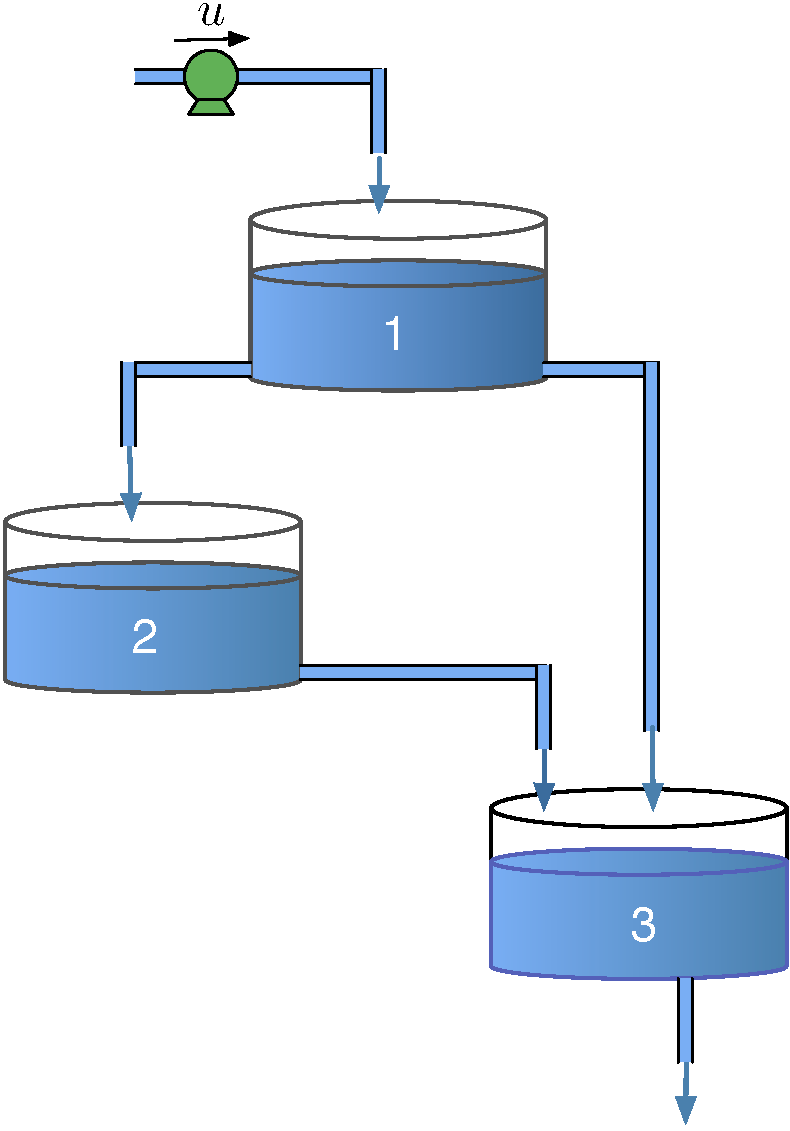
\includegraphics[width=7cm]{cascade}
\caption{Waterfall of tanks.}
\label{Fig:cascade}
\end{center} 
\end{figure}

It is clearly a compartment system whose the associated graph 
is depicted at figure \ref{Fig:grafassoc} and whose the continuity 
equations are written as~:
\begin{equation*} \begin{split} 
\dot x_1 &= q_{01} - q_{12} - q_{13} \\
\dot x_2 &=  q_{12} - q_{23} \\
\dot x_3 &= q_{13} + q_{23} - q_{30} 
\end{split} \end{equation*}
\begin{figure}[h] 
\begin{center}
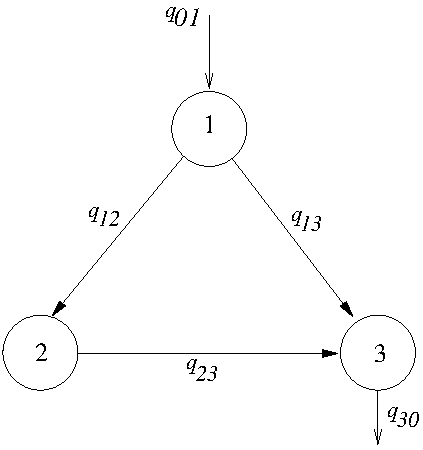
\includegraphics[width=7cm]{grafassoc}
\caption{Graph of the waterfall of tanks.}
\label{Fig:grafassoc}
\end{center} 
\end{figure}
In these equations, the sate variables $x_1$,$ x_2$ et $x_3$ specify, 
obviously, the volumes of water contained in the tanks; and the flows 
$q_{ij}$ depict the debits flowing from the upper tanks toward the lower 
tanks. In order to complete the model, the flows should be expressed in
terms of the sate variables and the input signals, correctly chosen.
The flow provided by the supply pomp of the upper tank can obviously be 
chosen as an input variable. The outgoing flow $q_{ij}$ of each tank 
is a positive function of the volume $x_i$ of the tank. The form of 
this function depends on the shape of the tanks and the configuration of 
the holes through which the water flows. Let's consider the case where the tanks 
have a constant horizontal section and where the flow goes through a 
rectangular hole located at the bottom of the tanks. The elevation of the water in 
a tank is expressed as~:
\eqnn
h_i = \frac {x_i}{S_i}
\eeqnn
where $S_{i}$ specifies the section of the tank.
According to the hydraulic laws, we know that when the elevation of the water $h_i$ is big 
toward the elevation of the hole, the link between the elevation of the water is proportional to 
$\sqrt{h_i}$ (Torricelli's law~\footnote{This law written by Torricelli in 1643 states that the speed $v$ of
the outgoing water of a tank of elevation $h$ verifies $v^2=2gh$. It can be proven intuitively by 
analogy with a body in free fall: a elementary volume of water at the surface of the tank has a potential energy 
$\rho g h$ and a kinetic energy $\rho v^2/2$ when it reaches the exit of the tank, where $\rho$ depicts the 
density. More rigorously, this can be deduced from Bernoulli's theorem without pressure loss or pump $p+\rho gz +\rho v^2/2 = \mathrm{constante}$, where $p$ depicts the pressure and $z$ the elevation.}). However, when the elevation of the water is lower than the elevation of the hole, the flows becomes proportional to $h_i\sqrt{h_i}$ 
(law of flows for a rectangular tank). A model of the following form can be given~:
\eqnn
q_{ij} = \frac { \alpha_{ij}h_i\sqrt{h_i} }{ \beta_{ij} + h_i}
\eeqnn
where $ \alpha_{ij}$ et $ \beta_{ij}$ are positive constants. Indeed, this model verifies the 
property telling that, for low water elevations ($h_i \ll \beta_{ij}$), the flow $q_{ij}$ is proportional to 
$h_i\sqrt{h_i}$ whereas for high water elevations ($h_i \gg \beta_{ij}$), the flow $q_{ij}$ is 
proportional to $\sqrt{h_i}$.
The flows $q_{ij}$ can be expressed in terms of $x_i$~:
\eqnn
q_{ij}(x_i) = \frac {k_{ij}x_i\sqrt{x_i} }{S_i \beta_{ij} + x_i} \hh \mbox{ avec } k_{ij} \triangleq \frac{\alpha_{ij}}{\sqrt{S_i}} 
\eeqnn
Finally, the state model can be written as~:
\begin{equation} \begin{split} \label{modetacasca}
\dot x_1 &= - \frac {k_{12}x_1\sqrt{x_1} }{S_1\beta_{12} + x_1} - \frac {k_{13}x_1\sqrt{x_1} }{S_1 \beta_{13} + x_1} + u, \\
\dot x_2 &=  \frac {k_{12}x_1\sqrt{x_1} }{S_1 \beta_{12} + x_1} - \frac {k_{23}x_2\sqrt{x_2} }{S_2 \beta_{23} + x_2},
\\
\dot x_3 &= \frac{k_{13}x_1\sqrt{x_1} }{S_1 \beta_{13} + x_1} + \frac {k_{23}x_2\sqrt{x_2} }{S_2 \beta_{23} + x_2} -
\frac {k_{30}x_3\sqrt{x_3} }{S_3 \beta_{30} + x_3}.
\end{split} \end{equation}
Let's notice that the functions $q_{ij}(x_{i})$ verifies the positivity conditions C1, C2 and C3. \qed
\end{exemple}


%%%%%%%%%%%%%%%%%%%%%%%%%%%%%%%%%%%%%%%%%%%%%%%%%%
%%%%%%%%%%%%%%%%%%%%%%%%%%%%%%%%%%%%%%%%%%%%%%%%%%
%%%%%%%%%%%%%%%%%%%%%%%%%%%%%%%%%%%%%%%%%%%%%%%%%%
%%%%%%% PARTIE DE DOUNIA MULDERS    %%%%%%%%%%%%%%
%%%%%%%%%%%%%%%%%%%%%%%%%%%%%%%%%%%%%%%%%%%%%%%%%%
%%%%%%%%%%%%%%%%%%%%%%%%%%%%%%%%%%%%%%%%%%%%%%%%%%
%%%%%%%%%%%%%%%%%%%%%%%%%%%%%%%%%%%%%%%%%%%%%%%%%%


\section{Linear models driven by controlled external supplies}

This is the most represented class of compartmental models within the literature.
It is characterized by the following flow definitions:
\begin{enumerate}
\item Flows between compartments and system output flows  are linear in function of the providing compartment level:
\eqnn
q_{ij} = k_{ij}x_i \hspace{1cm} k_{ij} > 0 \hspace{1cm} (i=1,...,n;j=0,...,n)
\eeqnn
\item The system inputs $u_{\ell}$ are proportional to the supply flow: 
\eqnn
q_{0\ell} = k_{0\ell}u_{\ell} 
\eeqnn
\end{enumerate}

In that case, the required information used to write the state model is entirely unclosed within the system graph.
The state model can be represented as a linear system (see chapter 1):
\eqnn
\dot{x} = Ax + Bu
\eeqnn
with the following structural features:
\begin{enumerate}
\item Matrix $A$ is a {\em Metzler matrix} i.e. such that $a_{ij} \geq 0$ for all $i \neq j$
\item Matrix $A$ is diagonally dominant i.e.
\eqnn |a_{ii}| \geq \sum_{j \neq i} a_{ji} 
\eeqnn
\item Matrix $B$ is a full rank {\em elementary matrix}, i.e. a matrix containing at most one non null element per line and per column.
\end{enumerate}

\begin{exemple}
The compartmental system linear state model corresponds to the graph shown on \ref{fig:exemplecomp} 
and can be written as:
\begin{equation} \begin{split}
\bma{c} \dot x_1 \\ \dot x_2 \\ \dot x_3 \ema &= 
\bma{ccc} -(k_{12} + k_{13}) & k_{21} & 0 \\ 
k_{12} & -(k_{21} + k_{23}) & 0 \\ k_{13} & k_{23} & - k_{30} \ema
\bma{c} x_1 \\ x_2 \\ x_3 \ema \\ &\hd
+ \bma{cc} k_{01} & 0 \\ 0 & k_{02} \\ 0 & 0 \ema
\bma{c} u_1 \\ u_2 \ema
\end{split} \end{equation}
We observe that $A$ is a diagonally dominant Metzler matrix and that $B$ is a full rank elementary matrix ($rank = 2$).
\cqfd
\end{exemple}

\begin{exemple}{\bf \em Physiological modelling}
Physiologists are often interested in describing and analyzing biological or chemical substance propagation within mammal body.
Those substances can stand for medicinal substances (Pharmacokinetic studies) or toxic substances voluntary or accidentally absorbed.
They can also be natural substances such as hormones or proteins.
Compartmental models are frequently used to process such studies: 
the mammal body is therefore represented as a more or less diversified group of interconnected vessels.

Let us consider the example on figure \ref{Fig:grapharmaco}.
\begin{figure}[ht] 
\begin{center}
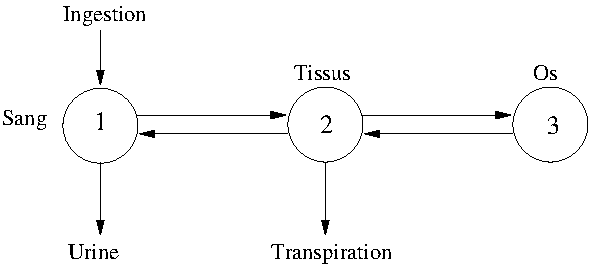
\includegraphics{grapharmaco}
\caption{Pharmacokinetic compartmental graph model}
\label{Fig:grapharmaco}
\end{center} 
\end{figure}

A toxic substance (lead for example) is absorbed by an animal and permeated in its blood.
This substance progressively propagates within the body, from the blood to tissues at first, towards bones afterwards.
It is secreted by sweating from one part and by urinating from the other part.
The linear compartmental model corresponding to the graph on figure \ref{Fig:grapharmaco} is the following model:
\begin{equation*} \begin{split}
\bma{c} \dot x_1 \\ \dot x_2 \\ \dot x_3 \ema &= 
\bma{ccc} -(k_{10} + k_{12}) & k_{21} & 0 \\ 
k_{12} & -(k_{20} + k_{21} + k_{23}) & k_{32} \\ 0 & k_{23} & - k_{32} \ema
\bma{c} x_1 \\ x_2 \\ x_3 \ema \\
& \hd + \bma{c} k_{ 01}\\ 0 \\ 0 \ema u.
\end{split} \end{equation*}
In this model, the state variables are: $x_1$, $x_2$ et $x_3$, which stands for toxial substance quantities within the three compartments (blood, tissues and bones).
The input variable $u$ stands for the body ingestion flow.
\cqfd
\end{exemple}


\section{Non linear model with controlled flows}
We will now consider non linear compartmental systems which flows $q_{ij}$ can be non linear functions whose arguments respect the C1 - C3 conditions.
We already approached a non linear model in the vessels cascade example.
However, flows between compartments were not depending on input variables $u_{\ell}$ in that example.
We will here consider a case where flows between compartments are explicit functions of input variables $u_{\ell}$ 
allowing to monitor the debit between compartments.
The symbolic representation presented on figure \ref{Fig:contflux} shows the presence of such a monitoring variable.
\begin{figure}[ht] 
\begin{center}
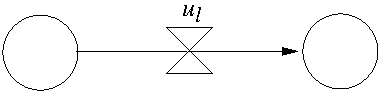
\includegraphics{contflux}
\caption{Symbolic representation of a monitored flow}
\label{Fig:contflux}
\end{center} 
\end{figure}


\begin{exemple}{\bf \em Vessels network}
Let us consider the hydraulic system represented on figure \ref{Fig:reseauh}. 
This vessels network corresponds to the vessel cascade example (\ref{systhyd} with a small modification:
the flow between vessel $2$ and vessel $3$ is now monitored by a pump.
As this pump is controllable, we can consider the pumped debit $F$ as an input variable.

\begin{figure}[h] 
\begin{center}
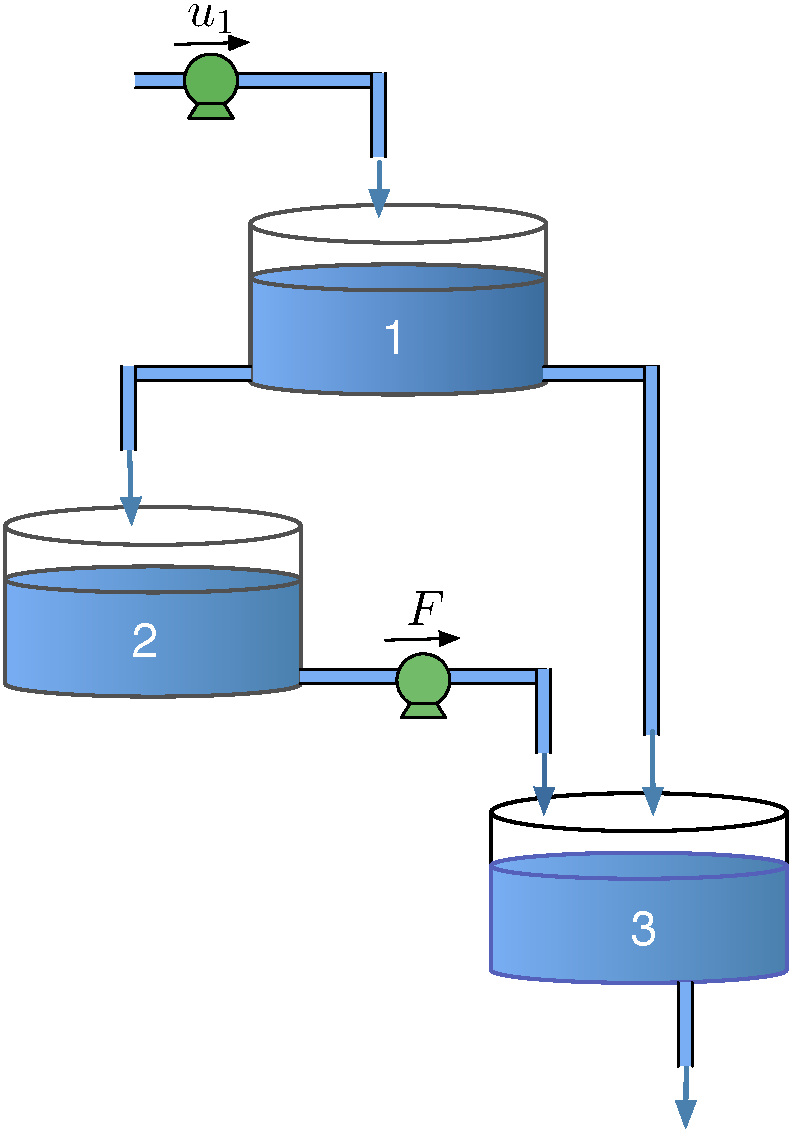
\includegraphics[width=7cm]{reseauh}
\caption{Vessels networks}
\label{Fig:reseauh}
\end{center} 
\end{figure}

The state model (\ref{modetacasca}) we obtained for the vessels cascade is therefore simply modified as follows:
\begin{equation} \begin{split}
\dot x_1 &= - q_{12}(x_1) - q_{13}(x_1) + u_1 \\
\dot x_2 &=  q_{12}(x_1) - u_2 \label{modres1} \\
\dot x_3 &= q_{13}(x_1) - q_{30}(x_3) + u_2 
\end{split} \end{equation}
where the state variables $x_i$ stand for water volumes contained in vessels,
input variable $u_1$ corresponds to the first vessel supply debit,
input variable $u_2 = F$ corresponds to the pumped flow from the second vessel towards the third vessel
and functions $q_{ij}(x_i)$ are defined as follows:
\eqnn
q_{ij}(x_i) = \frac {k_{ij}x_i\sqrt{x_i} }{S_i \beta_{ij} + x_i}
\eeqnn
We observe that this state model {\it cannot} represents a compartmental system respecting C1-C3 conditions.
The flow $q_{23} = u_2$ does indeed not respect the C3 condition and the system is not positive:
simulations of this model can lead to negative vessels levels (even if the pumped debits remain positive) 
which is obviously conflicting with physical reality.

The model as stated indeed allows to pump water in the second vessel even when it is empty!

This problem can be easily avoided if the flow $q_{23}$ (where the pumped debit is $F$) is modeled such as it respects the physical reality and 
the C3 condition as:
$$q_{23}(x_2,u_2) = \phi(x_2)u_2$$
where $\phi(x_2)$ is a positive function satisfying $\phi(0) = 0$ and
$u_2$ represents the pump activation.

We therefore obtain a compartment system which graph is presented on figure \ref{Fig:graphreseau} and the state model can be written as:

\begin{equation*} \begin{split}
\dot x_1 &= - q_{12}(x_1) - q_{13}(x_1) + u_1 \\
\dot x_2 &=  q_{12}(x_1) - \phi(x_2)u_2 \\
\dot x_3 &= q_{13}(x_1) - q_{30}(x_3) + \phi(x_{2})u_2 
\end{split} \end{equation*}
\begin{figure}[h] 
\begin{center}
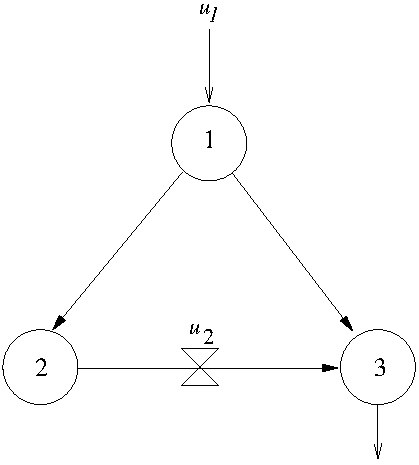
\includegraphics[width=7cm]{graphreseau}
\caption{Vessels network associated graph}
\label{Fig:graphreseau}
\end{center} 
\end{figure}
\cqfd
\end{exemple}
The fundamental structural property of compartments linear systems can be generalized to non linear system with the following theorem.

\begin{theoreme} 
Given a compartments non linear system which flows $q_{ij}$ satisfy C1-C3 conditions.
Therefore, the flows can be written as follows:
\eqnn
&& q_{ij}(x,u) = a_{ij}(x,u)x_i \hspace{4mm}
(i=1,...,n;j=1,...,n)\\ 
&& q_{i0}(x,u) = a_{i0}(x,u)x_i \hspace{4mm}
(i=1,...,n)\\
&& q_{0i} = k_{0i}u_i
\eeqnn
where functions $a_{ij}(x,u)$ et $a_{i0}(x,u)$, defined on the positive orthant, are continuous. 

Therefore, the system state model can be written as:
$$ \dot x = A(x,u)x + Bu $$
where the matrix $A(x,u)$ is a diagonally dominant Metzler matrix for all $(x,u)$ in the positive orthant 
and $B$ an elementary matrix.
\cqfd
\end{theoreme}

We will end this chapter with another industrial classical compartmental system example.

\begin{exemple}{\bf \em Binary distillation process}

A binary distillation process is a process used to split a liquid load composed of two liquid chemical components.
A {\it depropanizer} used to split propane from butane is a typical example of binary distillation process within the petrochemical industry.

The split is made by evaporation in an enclosed vessel called {\em round-bottom flask} (see figure \ref{Fig:distillation}).
\begin{figure}[h]
\begin{center}
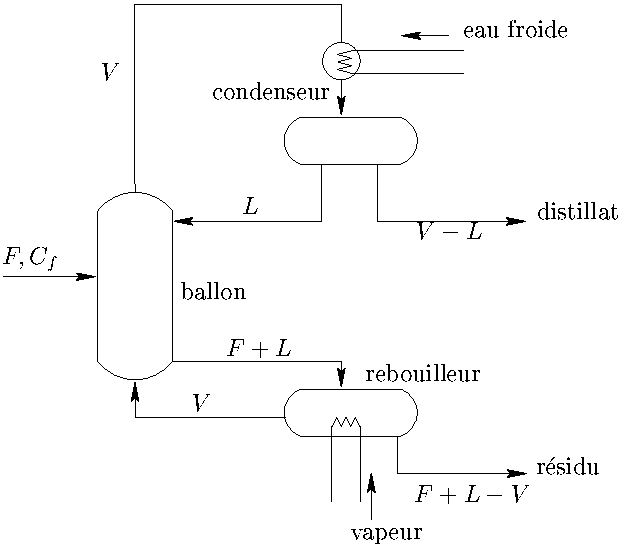
\includegraphics[width=8cm]{proc_distil}
\caption{Distillation process}
\label{Fig:distillation}
\end{center} 
\end{figure}
The {\it distillate} containing mainly the lightest component with a bit of the heaviest one exits from the top of the flask.

The {\it residue} containing mainly the heaviest component with a bit of the lightest one exits from the bottom of the flask.

The flask is filled by the liquid load with a molar debit $F$ (mol/min). 
The steam flow spreading out the flask is cooled down and entirely condensed.
The outgoing liquid is partially recycled toward the flask with a molar debit $L$. 

The remaining part, called {\it distillate}, is extracted from the system.

At the bottom of the flask, the outgoing liquid is warmed up a boiler and the produced steam is recycled within the flask.
The remaining part, called {\it residue}, is extracted from the system.

The distillation process dynamic is simplified by the following modeling assumptions and represented below:
\begin{enumerate}
\item the load is liquid and has the flask temperature;
\item the liquid and steam state in the flask and the boiler are homogeneous and at equilibrium;
\item the flask pressure is constant and there is no steam accumulation; this assumption allows to omit pressure dependencies
in the equations and implies that the steam debit $V$  exiting the flask is equivalent to the input debit; 
\item the liquid extraction debits are adjusted such as the total molar masses of the components in liquid state remain constant : 
the distillate is therefore extracted with a molar debit $V-L$, the liquid at the bottom of the flask is extracted with a molar debit $F+L$
and the residue is extracted with a molar debit $F+L-V$. Obviously, this implies that the inequality $0 < L < V < F+L$ has to be verified.\\
\end{enumerate}

Given this definition, the distillation process can be interpreted as a compartments system which dynamic model is based on
balance equations of one of the two components in the flask, in the condenser and in the boiler.
This compartments system graph is presented on figure \ref{Fig:graphdisti} and the state equations are:
\begin{equation*} \begin{split}
\dot x_1 &= u_2 k(x_2) - u_{1}\frac{x_1}{m_1} - (u_2 - u_1) \frac{x_1}{m_1}\\
\dot x_2 &= u_1\frac{x_1}{m_1} - (u_1+u_3)\frac{x_2}{m_2} + u_2(k(x_3) - k(x_2)) + u_3c_f\\
\dot x_3 &= (u_1 + u_3)(\frac{x_2}{m_2} - \frac{x_3}{m_3}) + u_2(\frac{x_3}{m_3} - k(x_3))
\end{split} \end{equation*}
\begin{figure}[h]
\begin{center}
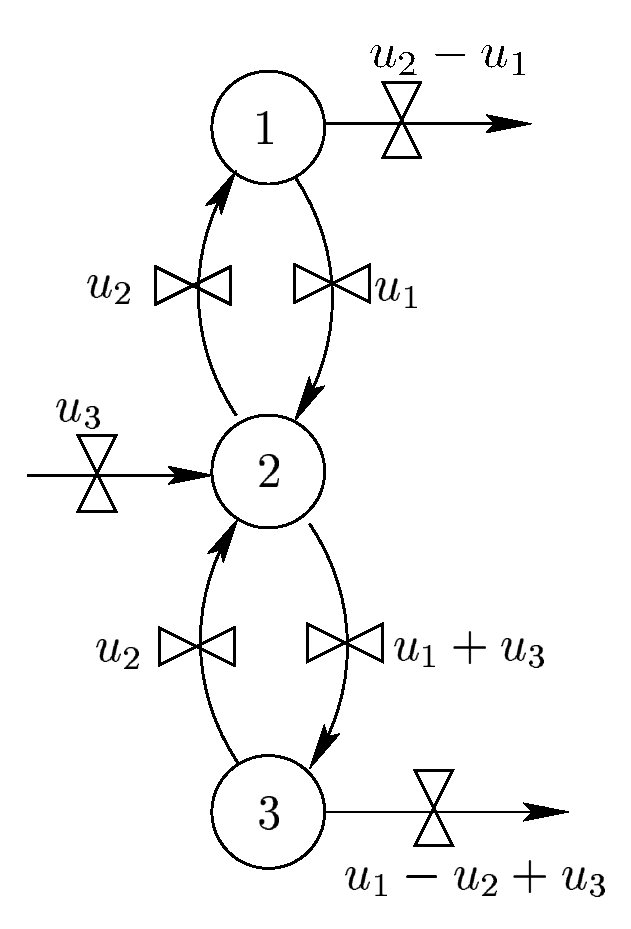
\includegraphics[width=5cm]{graphprocdistil}
\caption{Distillation process associated graph}
\label{Fig:graphdisti}
\end{center} 
\end{figure}
State variables $x_i$ stand for the molar mass of the lightest component in the liquid state within
the condenser (index $1$), the flask (index $2$) and the boiler(index  $3$);

Parameters $m_i$ represent those total (and constant) molar masses : 
the ratio $x_i/m_i$ corresponds to the {\it molar fraction}; 
parameter $c_f$ molar fraction of the lightest component within the load; 

Input variables $u_1 = L$, $u_2 = V$ and $u_3 = F$ are, respectively, molar debit of the reflux, the steam production and the supply.
Finally, the function $k(x)$ is a liquid-steam equilibrium relationship allowing to link the molar fraction of the lightest component
leaving the liquid by vaporization to the molar fraction of the component in liquid state. 
\begin{figure}[ht]
\begin{center}
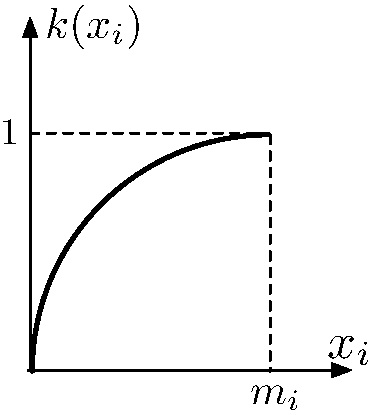
\includegraphics[width=4cm]{separ}
\caption{Liquid-steam equilibrium relationship}
\label{Fig:separ}
\end{center} 
\end{figure}

\noindent This relationship is classically expressed as follows:
\eqnn
k(x_i) \triangleq \frac{\alpha x_i}{m_i + (\alpha - 1)x_i}
\eeqnn
where the constant parameter $\alpha > 1$ is called separation factor.
This function, defined on the interval $[0,m_i]$, checks $k(0) = 0$ and
$k(m_i) = 1$ (see figure \ref{Fig:separ}). \qed  
\end{exemple}

\section{Exercises}

\begin{exercice}{\bf \em A compartments system}

Given the following dynamical system:
\begin{align*}
\dot x_{1} &= x_{3} - \log (1+x_{1}) \\
\dot x_{2} &= x_{3} - x_{2}^2 \\
\dot x_{3} &= x_{2}^2 - 2x_{3} + u
\end{align*}
Demonstrate that it is a compartments system. Draw the associated graph. Compute the flows $q_{ij}$, the matrix $L$ and the matrix $A(x,u)$. \qed
\end{exercice}
\vv

\begin{exercice}{\bf \em A hydraulic system}

A hydraulic system containing three vessels and two pumps is presented on figure \ref{Fig:systhydr}.
\begin{figure}[h]
\begin{center}
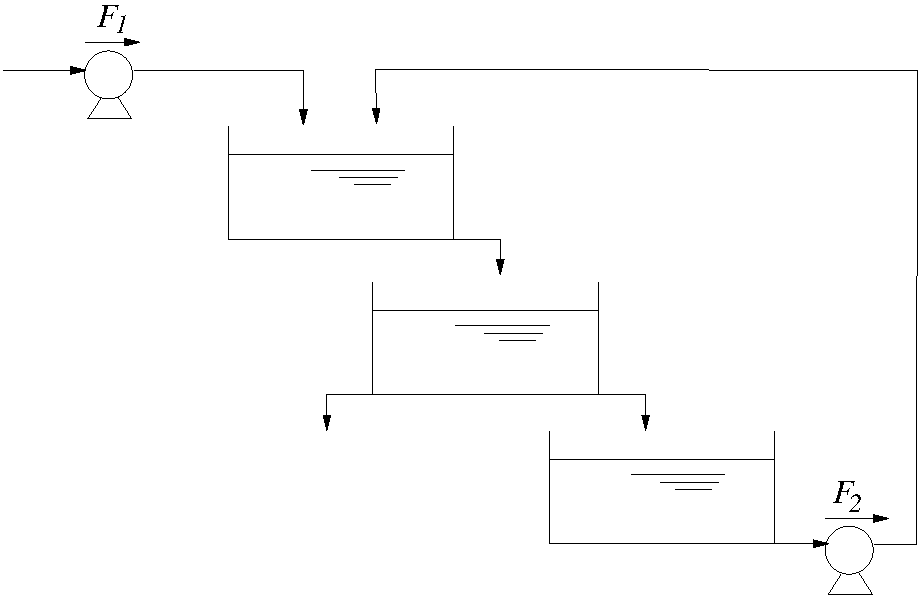
\includegraphics[width=8cm]{systhydr}
\caption{Hydraulic system}
\label{Fig:systhydr}
\end{center} 
\end{figure}
\begin{enumerate}
\item Establish a state model for the system, where the volumetric debits $u_1 = F_1$ and $u_2 = F_2$ are input variables. 
Show that the obtained system is {\it not} a positive system. 
\item Suggest an alternative definition for the input variable $u_2$ which ensure a postive system. 
\item Draw the obtained compartments graph model. \qed
\end{enumerate}
\end{exercice}
\vv 

\begin{figure}[!ht] 
\begin{center}
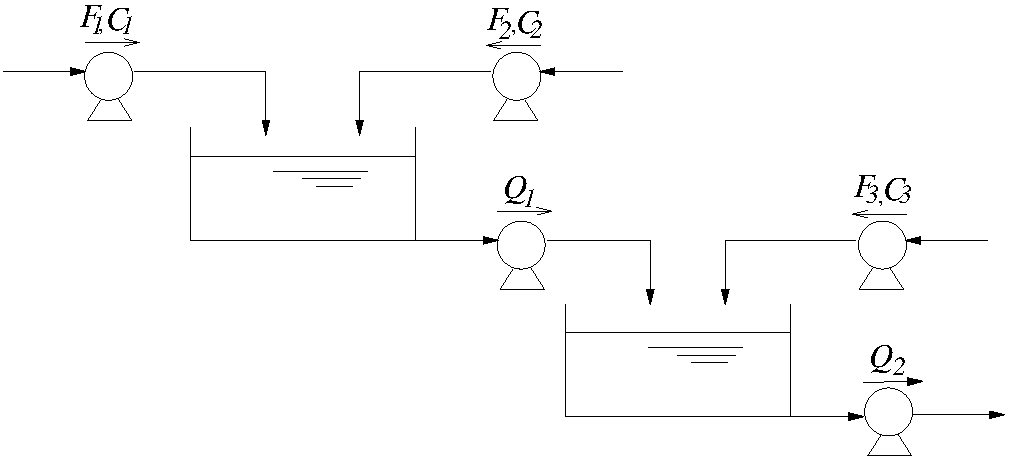
\includegraphics[width=8cm]{cuvmel}
\caption{Mixing vessels network}
\label{Fig:cuvmel}
\end{center} 
\end{figure}

\begin{exercice}{\bf \em A mixing vessels network}

The system represented on figure \ref{Fig:cuvmel} is designed for mixing three substances $X_1, X_2, X_3$ 
whose supply concentrations are denoted $C_1, C_2, C_3$ respectively.

The contained volumes in the two vessels are denoted $V_1$ and $V_2$. 
The pump volumetric debits are denoted as $Q_1, Q_2, F_1, F_2, F_3$.

\begin{enumerate}
\item Establish a state model of the system with the following input variables: 
$u_1 = Q_1/V_1, u_2 = Q_2/V_2, u_3 = C_1, u_4 = C_2, u_5 = C_3$. 
The debits $F_i$, $i = 1, \dots , 3$, are supposed constants.
\item Justify the input variables $u_1$ and $u_2$ form. \qed
\end{enumerate}
\end{exercice}
\vv

\begin{exercice}{\bf \em Compartments linear model}

Characterize the graph structure of a compartments linear model whose associated matrix $A$ is:
\begin{enumerate}
\item bidiagonal
\item tridiagonal
\item lower triangular \qed
\end{enumerate}
\end{exercice}
\vv

\begin{exercice}{\bf \em Distillation process model}

Determine the matrix $A(x,u)$ of the distillation process model. \qed
\end{exercice}
\vv

\begin{exercice}{\bf \em Communicating vessels}

A system with two communicating vessels is represented on figure \ref{Fig:reservoircom}.
The liquid flows freely between the two vessels and towards the outside under the hydrostatic pressure action.

\begin{figure}[h]
\begin{center}
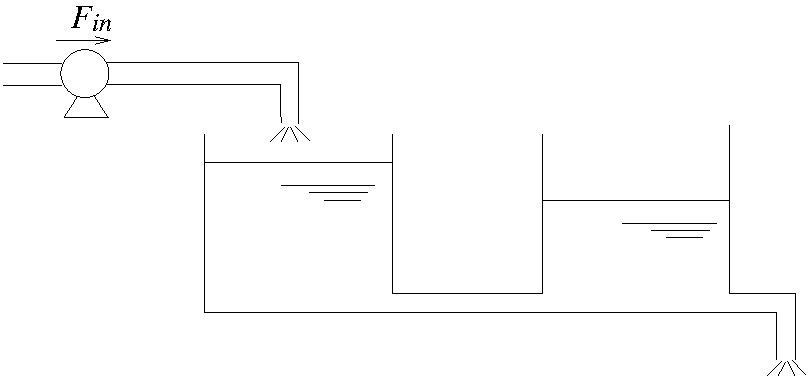
\includegraphics[width=8cm]{reservoircom}
\caption{Communicating vessels}
\label{Fig:reservoircom}
\end{center} 
\end{figure}

\begin{enumerate}
\item Establish a state model of the system. The provided debit (by the supply pump) is the only input variable. 
\item Show that it is a compartments system. Draw the associated graph. Explain the flow between the compartments. \qed
\end{enumerate}
\end{exercice}

\end{document}
